% !TEX root = ../main.tex

% 中英标题:\chapter{中文标题}[英文标题]
\chapter{多元时间序列异常检测相关背景技术介绍}[Typesetting pictures]

\section{引言}[Introduction]
本章是多元时间序列异常检测相关背景技术介绍。首先在第一节介绍了什么是时间序列中的异常,即时间序列异常的相关类型,包括全局异常、上下文异常、季节性异常、趋势异常、Shapelet异常等,并通过具体的例子与公式对其进行了详细的解释。然后在第二节和第三节介绍了多元时间序列异常检测的相关技术。在第二节主要介绍了基于预测的多元时间序列异常检测技术及应用,分别介绍了基于RNN的方法、基于GNN的方法以及基于Transformer的方法。在第三节主要介绍了基于重构的多元时间序列异常检测技术,分别介绍了基于AE的方法、基于GAN的方法以及基于Transformer的方法。

\section{多元时序数据的异常类型与异常定义方法}[Doctoral picture example]
根据Hawkings\cite{hawkings}对异常的定义 ,异常是指偏离一般分布的数据,如单个观测(点)或一系列观测(子序列) ,大大偏离一般分布。往往只有数据集中的很小一部分数据有异常,这通常意味着数据集是正态分布的。同时在真实世界的数据中可能有相当大量的噪音,这些噪音可能会对研究人员造成干扰,所以最有意义的偏差通常是那些明显不同于常规的偏差。在存在噪声的情况下,数据的主要特征是相同的。

时间序列中的异常可以分为时序异常(Temporal anomalies)、指标间异常(inter-metric anomalies)或时序-指标间异常(temporal inter-metric anomalies)\cite{aiops2022}。在一个单维时间序列中,时序异常可以是偏离与它相邻的子序列(local anomlies),也可以是偏离其整个整体序列(global anomlies),时序异常的例子可见图xxx。
时间异常也可能发生在多维时间序列中,并可能影响多个维度或所有维度。随着时间的推移,当一种异常的行为模式出现时,可能会出现后续的异常现象; 然而,每个观察结果本身可能并不会被认为是一次异常。例如,作为一个点异常的结果,导致该异常产生的事件可能发生在一个时间点,故此时异常被认为是一段短子序列。更具体的,不同类型的时序异常定义如下:

\textbf{全局异常(Global)}: 它们是序列中的峰值,与序列的其余部分相比,它们是具有极端值的点。例如,一个全球性的反常现象是,客户在一个典型的日子里支付了一笔异乎寻常的大额费用。考虑一个阈值threshold,它可以描述为:
\begin{equation}
    \left|x_t-\hat{x}_t\right|>\text { threshold }
    \end{equation}
其中 $\hat{x}$ 是模型的输出。如果输出值和实际点之间的差值大于阈值,则认为这是异常现象。

\textbf{上下文异常(Contextual)}: 某个时间点观测值偏离上下文。这里上下文定义为位于一定范围内的相邻时间点。这些类型的离群值是连续数据中的小故障,它们的值偏离了它们相邻的观察值。一个点可以是在一个上下文中是正常的,而在另一个上下文中是异常的。例如网络流量突然增加,在特定节日或特定时刻,被认为是正常的该公式与全局异常的公式相同,但阈值不同由上下文观察值决定:
\begin{equation}
    \text { threshold } \approx \lambda * \operatorname{var}\left(X_{t-w}:_{t+w}\right)
    \end{equation}
其中$X_{t-w}: t+w$ 指数据点$x_t$的上下文,窗口大小$w$, $var$是数据点上下文的方差,$\lambda$控制阈值的系数。

\textbf{季节性异常(Seasonal)}: 季节性异常的例子中,时间序列的形状和趋势可能相似,但它们的季节性与整体季节性相比可能出现偏差。例如一个餐馆在一周内的每日顾客人数。这样一个子序列有一个明确的每周季节性,寻找这种季节性的偏差并单独处理异常周期是有意义的:
\begin{equation}
    \operatorname{diss}_S(S, \hat{S})>\text { threshold }
    \end{equation}
其中 ${diss}_S $是度量两个子序列之间差异的函数,$\hat{S}$ 表示期望子序列的季节性。

\textbf{趋势异常(Trend)}: 趋势异常值引起数据向其平均值永久转移,并导致时间序列趋势转变。这种异常保持了它的周期性和正常的季节性,但是它极大地改变了它的斜率。趋势有时会改变方向,这意味着它们可能从增加变为减少,反之亦然。例如图xxx中趋势改变的部分,被认为是趋势异常:
\begin{equation}
    \operatorname{diss}_t(T, \hat{T})>\text { threshold }
    \end{equation}
其中$\hat{T}$指的是正常序列的趋势。

\textbf{Shapelet异常}:Shapelet由Ye等人\cite{shapelet}提出,是一种描述时间序列中某个特定类别的形状的特征度量。Shapelet异常指的是时间序列中某个子序列的该特征偏离正常类别的Shapelet特征:
\begin{equation}
    \operatorname{diss}_c(C, \hat{C})>\text { threshold }
    \end{equation}
其中$\hat{C}$值的是正常类别的Shapelet特征。
\begin{figure}[htb]
    \centering
    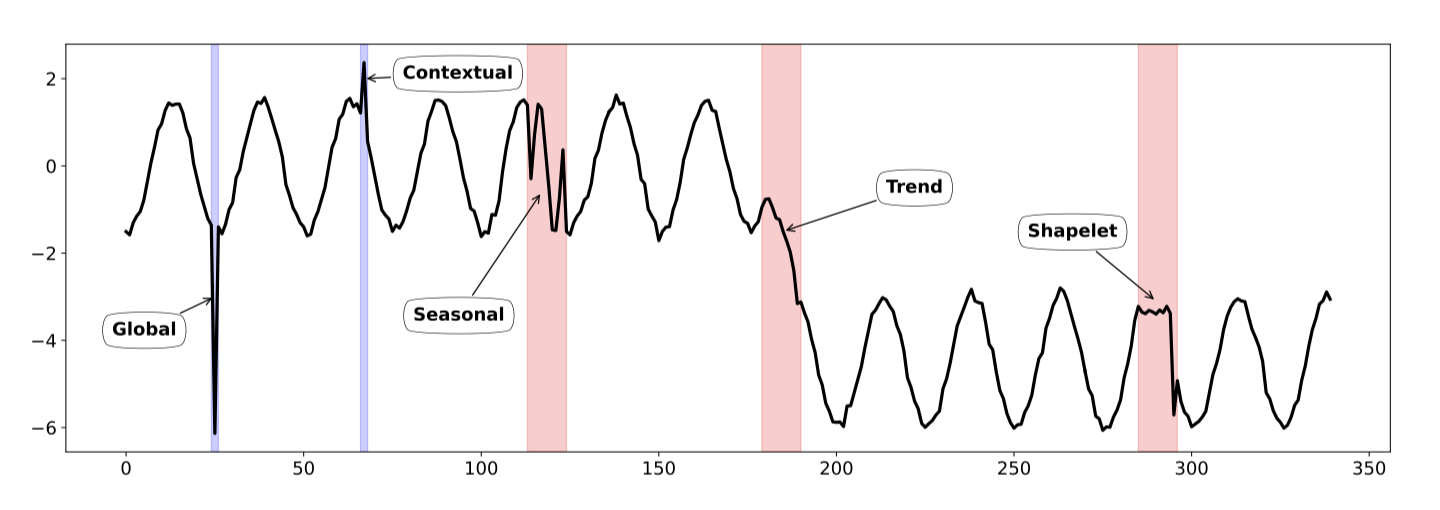
\includegraphics[width = 1\textwidth]{chapter2/untsano.jpg}
    \caption{单指标异常类别}
    \end{figure}
多元时间序列由多个维度(或称多个指标)组成,每个维度描述复杂实体的不同方面。一个实体的之间的空间依赖(相关性)也称为指标间依赖,可以是线性或非线性的。如果这些相关性被打破,多元时间序列将表现出广泛的异常行为。在图xxx的左边部分显示了一个例子,功耗(指标1)和 CPU 使用(指标2)之间的相关性是正的,但是它在开始后大约100秒。这种异常在本章中被称为指标间异常(inter-metric anomlies):
\begin{equation}
    \operatorname{diss}_{\text {corr }}\left(\operatorname{corr}\left(X^j, X^k\right), \operatorname{corr}\left(X_{t: t+w}^j, X_{t: t+w}^k\right)\right)>\text { threshold }
    \end{equation}
其中 $X^j$和 $X^k$ 是 多元时间序列 的两个不同指标,它们是相关的,并且 $corr$ 函数度量两个指标之间的相关性。当这种相关性在 $t: t + w$ 窗口中恶化时,这意味着系数偏离正常系数的程度大于阈值。

从时序异常或指标间异常的角度来看,时序指标间异常更容易检测,因为它们同时违反了时序异常和指标间异常,如图xxx右侧所示。
\begin{figure}[ht]
    \centering
    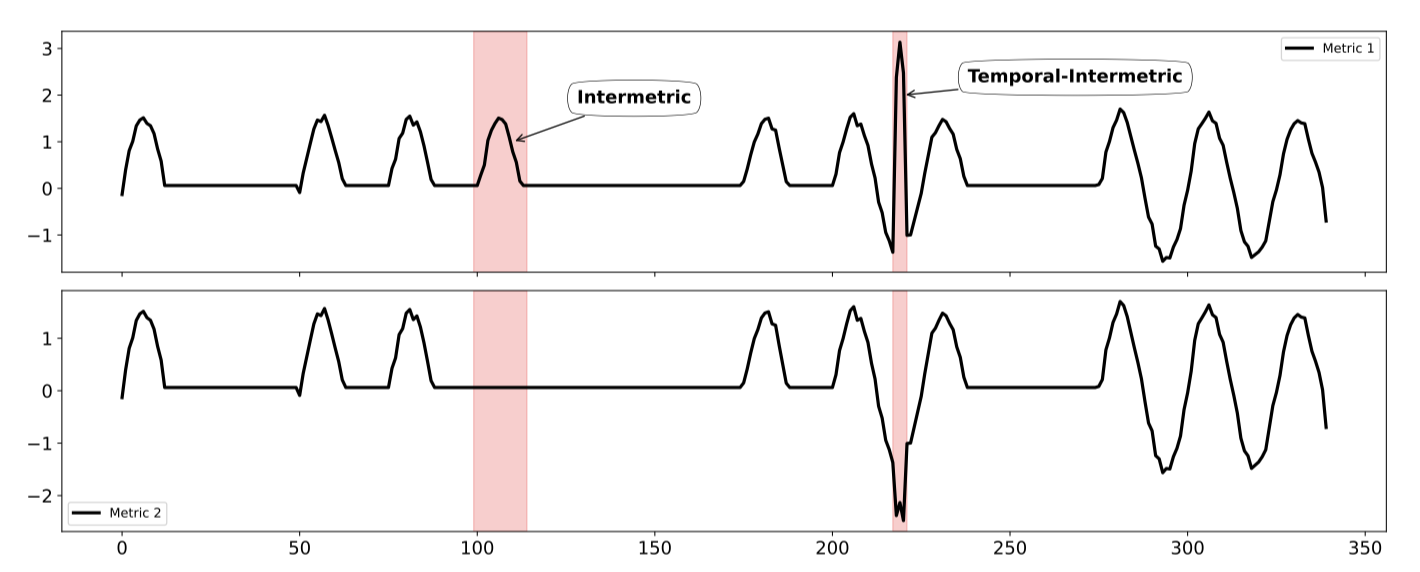
\includegraphics[width = 1\textwidth]{chapter2/mtsano.jpg}
    \centering
    \caption{多元时间序列的指标间异常和时序-指标间异常。在这个图中,指标1是功耗,指标2是 CPU 使用率\cite{aiops2022}}
    \end{figure}

\section{基于预测的多元时间序列异常检测相关技术}
基于预测的方法值的是使用一个学习好的模型,根据一个点或最近的窗口作为输入,预测下一个点或子序列,将预测值与实际值进行比较,确定传入值的异常程度。它们与实际值的偏差被认为是异常分数。大多数预测方法使用滑动窗口一次预测一个点的方式,为了识别异常行为,他们使用一个预测器来模拟正常行为。其中基于预测的方法根据其技术又可分为基于RNN的方法、基于GNN的方法以及基于Transformer的方法。下文介绍方法中,LSTM-NDT、Omnianomaly属于基于LSTM的方法;DeepAnt属于基于CNN的方法;GDN属于基于GDN的方法;GTA属于基于Transformer的方法。

\subsection{基于RNN的时间序列预测异常检测技术}
LSTM-NDT\cite{lstm-ndt}方法依赖于基于LSTM的深神经网络模型,该模型将输入序列用作训练数据,并且对于每个输入时间戳,预测了下一个时间戳的数据。LSTM-NDT是自动回归神经网络,在顺序数据中学习顺序依赖性,在每个时间戳上的预测都会使用上一个时间戳的输出中的反馈。这项工作还提出了一种非参数动态误差阈值(NDT)策略,以使用误差序列的移动平均值设置异常标记的阈值。但是,作为一个经常性模型,在许多情况下,这种模型的训练速度很慢。此外,LSTM通常在建模长的时间模式时效率低下,尤其是当数据嘈杂时。
% \begin{figure}[htb]
%     \centering
%     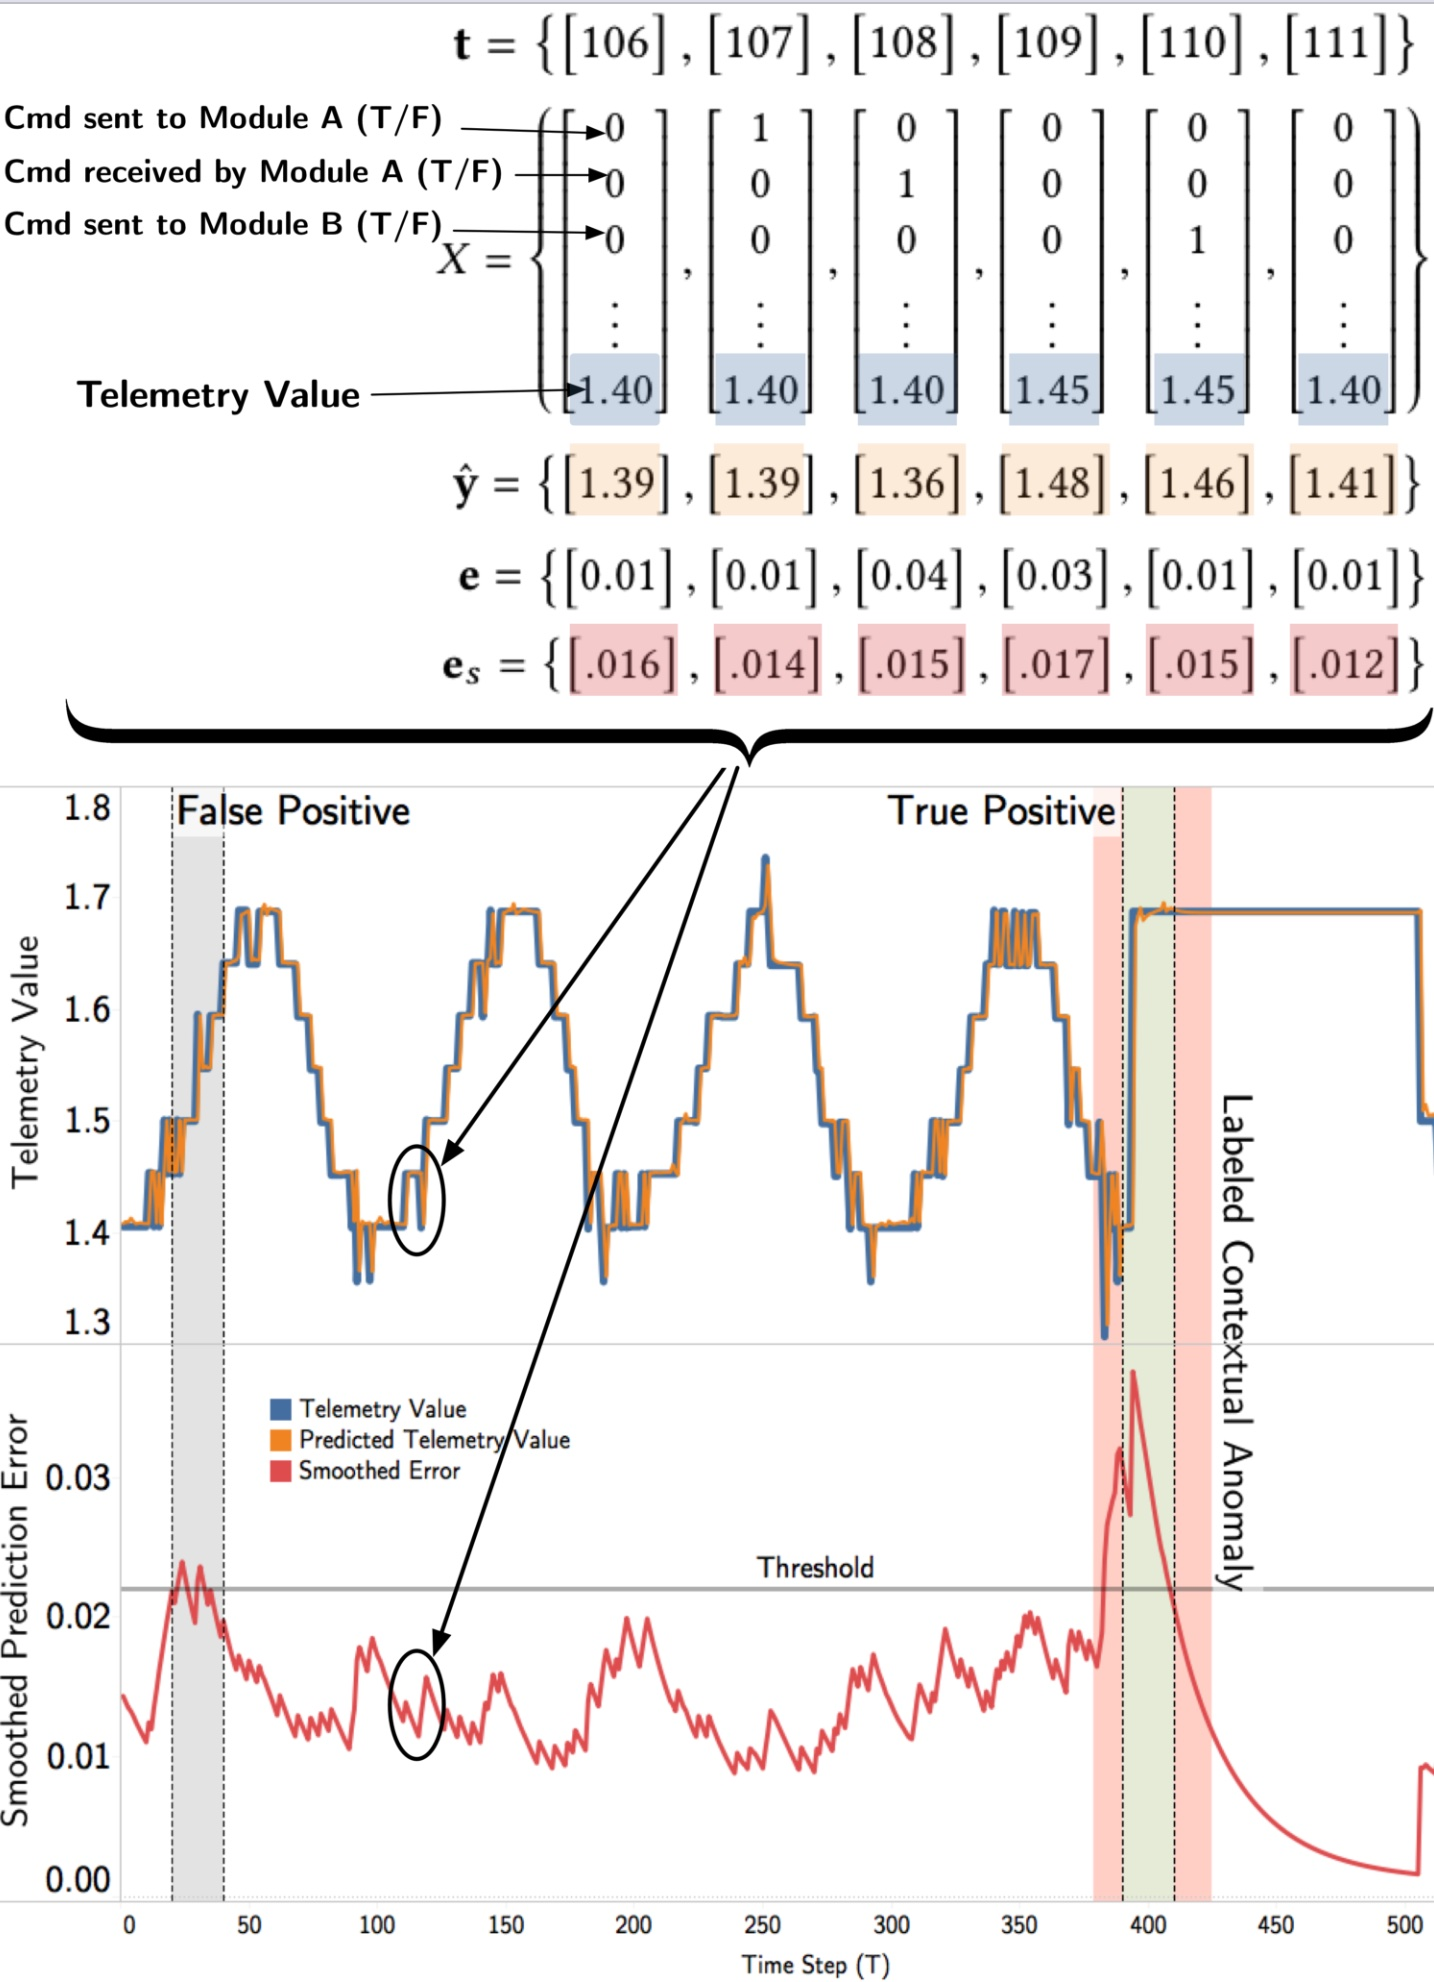
\includegraphics[width = 0.8\textwidth]{chapter1/lstm-ndt.jpg}
%     \caption{LSTM-NDT 模型架构\cite{lstm-ndt}}
%     \end{figure}

Omnianomaly\cite{Omnianomaly}是一种基于GRU与VAE结合的模型,其中提出一种随机回归神经网络来学习多变量数据的鲁棒表示,并且使用平面归一化流\cite{realnvp}来描述潜在空间的非高斯分布。该方法根据重建概率计算异常检测,并根据重建概率量化每个特征的可解释性。最后,该方法还实现了 POT 方法来寻找异常阈值,优于先前使用的NDT方法。具体来说: 对于长度为$N$的时间序列$\mathbf{X}=\left\{\mathbf{x}_1, \mathbf{x}_2, \ldots, \mathbf{x}_{\mathrm{N}}\right\}$,任意时刻$t$存在$M$维的观察向量$\mathbf{x}_{\mathbf{t}}=\left[x_t^1, x_t^2, \ldots, x_t^{\mathrm{M}}\right]$。Omnianomaly包含两个模块,即离线训练模块和在线检测模块,训练时,Omnianomaly中的pnet负责将$x_t$表示为潜在空间中的$z_t$, qnet负责将$z_t$重新生成$x_t$。

% Then, $\mathbf{e}_{\mathbf{t}}$, concatenated with $\mathbf{z}_{\mathbf{t}-1}$, enters the dense layer to generate mean $\mu_{\mathrm{z}_{\mathrm{t}}}$ and standard deviation $\sigma_{\mathrm{z}_{\mathrm{t}}}$ for the stochastic variable $\mathbf{z}_{\mathbf{t}}$ (Eq. 3b and 3c). As a result, z-space variables are now temporally dependent, as shown in Fig. 3(a1). The qnet can be formulated as follows:
在时间 $t$ 时,输入观测值 $\mathbf{x}_{\mathbf{t}}$  和 $\mathbf{e}_{\mathbf{t}-1}$(时刻 $t-1$ 时 GRU 中的隐变量)被发送到 GRU 单元,以生成隐变量 $\mathbf{e}_{\mathbf{t}}$。确定性 $\mathbf{e}_{\mathbf{t}}$ 对于全异常捕获  $\mathbf{x}_{\mathbf{t}}$ 与其前面的 $\mathbf{x}$ 空间观测之间的长期复杂时间信息至关重要。然后,$\mathbf{e}_{\mathbf{t}}$ 与 $\mathbf{z}_{\mathbf{t}-1}$ 连接,进入Dense Layer平均值$\mu_{\mathrm{z}_{\mathrm{t}}}$和标准差$\sigma_{\mathrm{z}_{\mathrm{t}}}$ ,因此,z-空间变量现在是时间相关的。Qnet 的表述如下:
\begin{equation}
    \begin{aligned}
    \mathbf{e}_{\mathrm{t}} & =\left(1-\mathbf{c}_{\mathrm{t}}^{\mathrm{e}}\right) \circ \tanh \left(\mathbf{w}^{\mathrm{e}} \mathbf{x}_{\mathbf{t}}+\mathbf{u}^{\mathrm{e}}\left(\mathbf{r}_{\mathbf{t}}^{\mathrm{e}} \circ \mathbf{e}_{\mathrm{t}-1}\right)+\mathbf{b}^{\mathrm{e}}\right)+\mathbf{c}_{\mathbf{t}}^{\mathrm{e}} \circ \mathbf{e}_{\mathrm{t}-1} \\
    \mu_{\mathrm{z}_{\mathrm{t}}} & =\mathbf{w}^{\mu_{\mathrm{z}}} h^\phi\left(\left[\mathbf{z}_{\mathrm{t}-1}, \mathbf{e}_{\mathrm{t}}\right]\right)+\mathbf{b}^{\mu_{\mathrm{z}}} \\
    \sigma_{\mathrm{z}_{\mathrm{t}}} & =\operatorname{softplus}\left(\mathbf{w}^{\sigma_{\mathrm{z}}} h^\phi\left(\left[\mathbf{z}_{\mathrm{t}-1}, \mathbf{e}_{\mathrm{t}}\right]\right)+\mathbf{b}^{\sigma_{\mathrm{z}}}\right)+\boldsymbol{\epsilon}^{\sigma_{\mathrm{z}}}
    \end{aligned}
    \end{equation}

$\mathbf{r}_{\mathbf{t}}^{\mathbf{e}}=\operatorname{sigmod}\left(\mathbf{w}^{\mathbf{r}^{\mathrm{e}}} \mathbf{x}_{\mathbf{t}}+\mathbf{u}^{\mathbf{r}^{\mathrm{e}}} \mathbf{e}_{\mathbf{t}-1}+\mathbf{b}^{\mathbf{r}^{\mathrm{e}}}\right)$ 是重置门,确定如何将新输入与先前的内存结合。 $\mathbf{c}_{\mathbf{t}}^{\mathbf{e}}=\operatorname{sigmod}\left(\mathbf{w}^{\mathbf{c}^{\mathbf{e}}} \mathbf{x}_{\mathbf{t}}+\mathbf{u}^{\mathbf{c}^{\mathbf{e}}} \mathbf{e}_{\mathbf{t}-\mathbf{1}}+\mathbf{b}^{\mathbf{c}^{\mathbf{e}}}\right)$ 是更新门决定保留多少以前的内存。

pnet试图使用类似于qnet的结构用$\mathbf{x}_{\mathbf{t}}$ 重建$x_t$。作者利用线性高斯SSM来连接qnet中的z空间变量,并使它们具有时间依赖性:$\mathbf{z}_{\mathbf{t}}=\mathbf{O}_{\boldsymbol{\theta}}\left(\mathrm{T}_{\boldsymbol{\theta}} \mathbf{z}_{\mathbf{t}-1}+\mathbf{v}_{\mathbf{t}}\right)+\boldsymbol{\epsilon}_{\mathbf{t}}$, where $\mathbf{T}_{\boldsymbol{\theta}}$ and $\mathbf{O}_{\boldsymbol{\theta}}$ ,其中 $\mathbf{v}_{\mathbf{t}}$和$\boldsymbol{\epsilon}_{\mathbf{t}}$是跃迁和观测矩阵,v t和εt是跃迁和观察噪声。在时间$t, z_t$,以及变量$d_{t-1}$通过GRU单元以产生确定性变量$d_t$(等式4a)。然后通过致密层进一步处理$\mathbf{d}_{\mathbf{t}}$ ,以生成变量$\mathbf{x}_{\mathbf{t}}^{\prime}$的平均$\mu_{\mathbf{x}_{\mathrm{t}}}$ 和标准偏差$\sigma_{\mathbf{x}_t}$($\mathbf{x}_{\mathbf{t}}$的重建)。
\begin{equation}
    \begin{aligned}
    & \mathbf{d}_{\mathrm{t}}=\left(1-\mathbf{c}_{\mathbf{t}}^{\mathrm{d}}\right) \circ \tanh \left(\mathbf{w}^{\mathrm{d}} \mathbf{z}_{\mathrm{t}}+\mathbf{u}^{\mathrm{d}}\left(\mathbf{r}_{\mathrm{t}}^{\mathrm{d}} \circ \mathbf{d}_{\mathrm{t}-1}\right)+\mathbf{b}^{\mathrm{d}}\right)+\mathbf{c}_t^{\mathrm{d}} \circ \mathbf{d}_{\mathrm{t}-1} \\
    & \boldsymbol{\mu}_{\mathrm{x}_{\mathrm{t}}}=\mathrm{w}^{\boldsymbol{\mu}_{\mathrm{x}}} \boldsymbol{h}^\theta\left(\mathrm{d}_{\mathrm{t}}\right)+\mathbf{b}^{\boldsymbol{\mu}_{\mathrm{x}}} \\
    & \sigma_{\mathbf{x}_{\mathbf{t}}}=\operatorname{softplus}\left(\mathbf{w}^{\sigma_{\mathbf{x}}} h^\theta\left(\mathbf{d}_{\mathbf{t}}\right)+\mathbf{b}^{\sigma_{\mathbf{x}}}\right)+\epsilon^{\sigma_{\mathbf{x}}} 
    \end{aligned}
    \end{equation}
其中 $\mathbf{r}_{\mathbf{t}}^{\mathbf{d}}=\operatorname{sigmod}\left(\mathbf{w}^{\mathbf{r}^{\mathrm{d}}} \mathbf{z}_{\mathbf{t}}+\mathbf{u}^{\mathbf{r}^{\mathrm{d}}} \mathbf{d}_{\mathbf{t}-\mathbf{1}}+\mathbf{b}^{\mathbf{r}^{\mathrm{d}}}\right)$ 和 $\mathbf{c}_{\mathbf{t}}^{\mathbf{d}}=\operatorname{sigmod}\left(\mathbf{w}^{\mathbf{c}^{\mathrm{d}}} \mathbf{z}_{\mathbf{t}}+\right.$ $\mathbf{u}^{\mathbf{c}^{\mathrm{d}}} \mathbf{d}_{\mathbf{t}-1}+\mathbf{b}^{\mathbf{c}^{\mathrm{d}}}$, 它们分别是复位门和更新门。

% DeepAnt\cite{deep-ant}模型在训练阶段不需要大量数据,因此是有效的。该模型能够检测到时间序列模式中的小偏差,并且能够以无监督的方式处理低水平的数据污染(小于5\%)。异常检测模型可以应用于单变量和多变量时间序列,它可以识别异常,如点异常,上下文异常和不一致。
% \begin{figure}[htb]
%     \centering
%     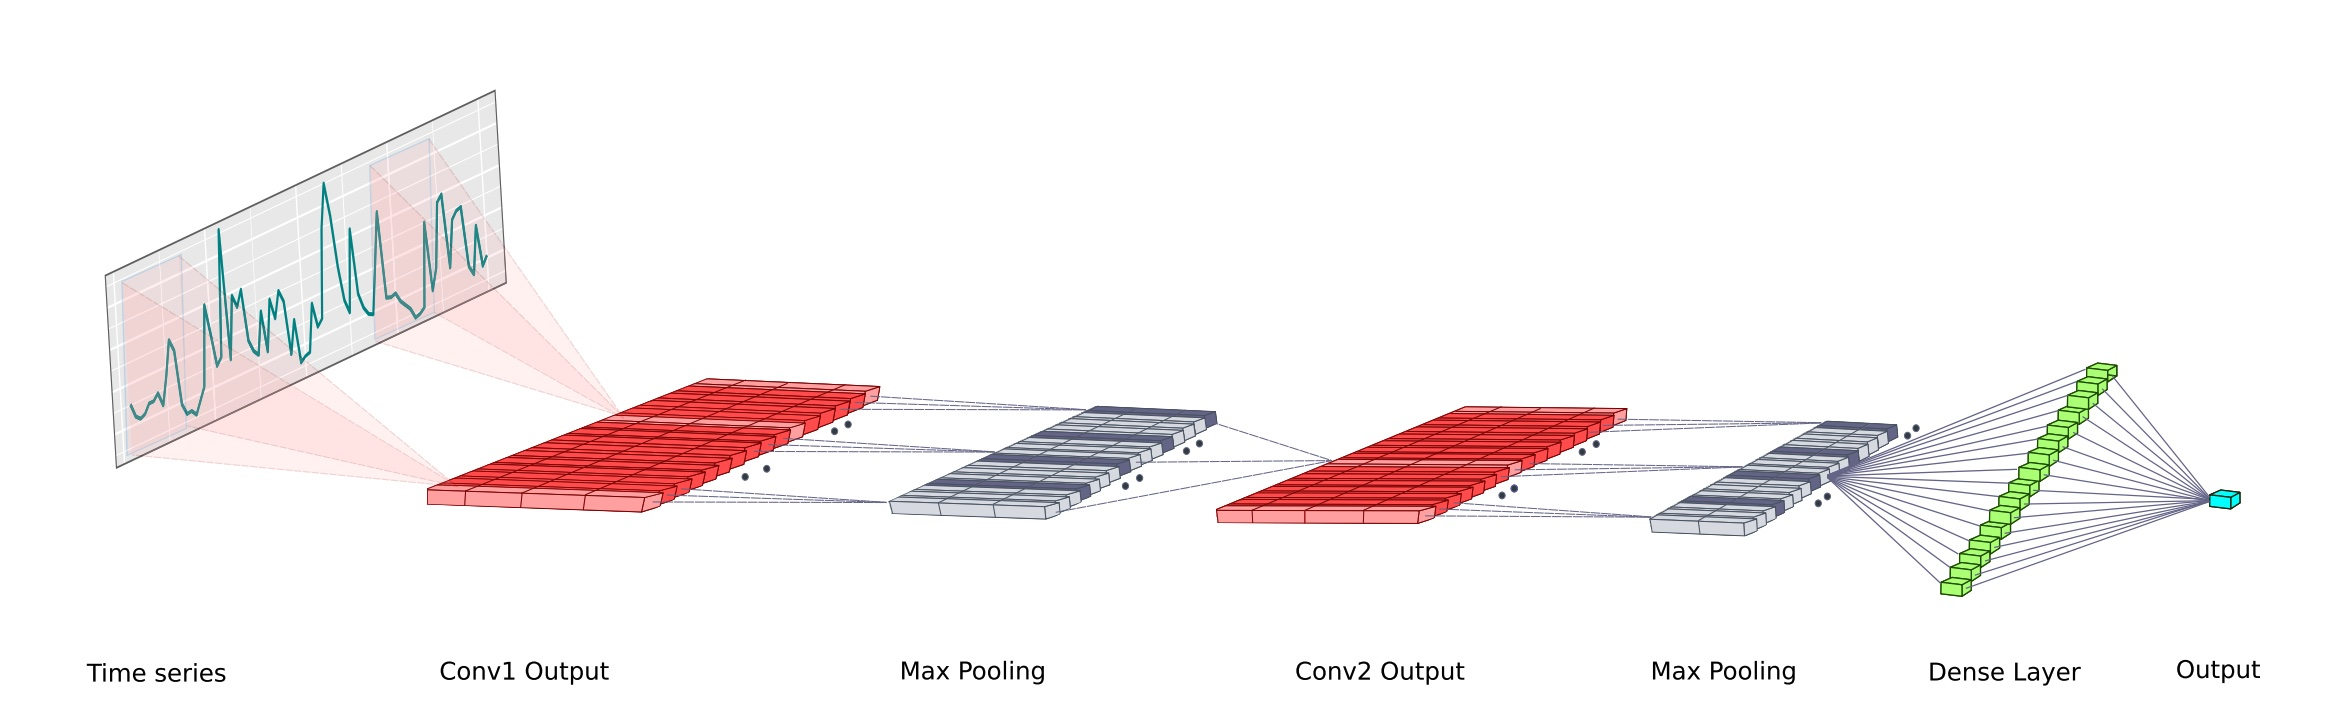
\includegraphics[width = 1\textwidth]{chapter1/deepant.jpg}
%     \caption{DeepAnt 模型架构\cite{deep-ant}}
%     \end{figure}
\subsection{基于GNN的时间序列预测异常检测技术}
Deng 等人\cite{gdn}于2021年在AAAI会议上发表了GDN模型。GDN采用 GNN 的方法捕捉多个时间序列之间的关联关系,并通过一个全连接层对未来时刻的数据进行预测,以预测值与真实值之间的差异作为异常分数进行异常检测,这种方法更侧重于多元之间序列之间的相关性特征进行建模。如图1-2所示,GDN主要包括4个部分,即传感器嵌入, 图结构学习,基于图注意力的预测以及图偏差评分。其中传感器嵌入主要利用嵌入向量捕获每个传感器的独特特性;图结构学习: 学习表示传感器之间依赖关系的图结构;基于图形注意力的预测: 基于图形注意力函数对各传感器的未来值进行预测;图偏差评分: 识别学习关系的偏差,并定位和解释这些偏差。
作者在传感器编码的过程中,将每个传感器用一个 embedding vector 来进行表示:
\begin{equation}
    \mathbf{v}_{\mathbf{i}} \in \mathbb{R}^d, \text { for } i \in\{1,2, \cdots, N\}
    \end{equation}
考虑到不同 传感器 间依赖模式是不对称的, 论文中利用有向图来表示 传感器 间的关系, 其 对应的邻接矩阵为 $A_{i j}$ 。对于每个 sensor $i$ 其依赖的 condidate relations 为 $\mathcal{C}_i \subseteq\{1,2, \cdots, N\} \backslash\{i\}$ 。如果有先验知识 那么 $\mathcal{C}_i$ 可以自定义, 如果没有那么为除本身外的全集。为了选择 sensor $i$ 的依赖, 需要计算其对于每个 condidate relations 中 $j \in \mathcal{C}$ 的相似性:
\begin{equation}
    \begin{aligned}
    e_{j i} & =\frac{\mathbf{v}_{\mathbf{i}}^{\top} \mathbf{v}_{\mathbf{j}}}{\left\|\mathbf{v}_{\mathbf{i}}\right\| \cdot\left\|\mathbf{v}_{\mathbf{j}}\right\|} \text { for } j \in \mathcal{C}_i \\
    A_{j i} & =\mathbf{1}\left\{j \in \operatorname{TopK}\left(\left\{e_{k i}: k \in \mathcal{C}_i\right\}\right)\right\}
    \end{aligned}
    \end{equation}
然后选择 top-k 个最相似的作为其依赖 sensor,k 值根据稀疏性进行判断。在时刻 $t$ 模型输入为 $\mathbf{x}^{(t)} \in \mathbb{R}^{N \times w}$, 其 $w$ 表示历史序列时间窗口, 目标是需要判断在当前时刻值 $\mathbf{S}^{(t)}$
$$
\mathbf{x}^{(t)}:=\left[\mathbf{s}^{(\mathbf{t}-\mathbf{w})}, \mathbf{s}^{(\mathbf{t}-\mathbf{w}+\mathbf{1})}, \cdots, \mathbf{s}^{(\mathbf{t}-\mathbf{1})}\right]
$$
为了考虑 sensor 间的关系, 论文中采用图注意力机制来融合 sensor 特征 $\mathbf{v}_{\mathbf{i}}$, 对于节点 $i$ 聚合特 征 $\mathbf{z}_{\mathbf{i}}$ 计算方法如下及注意力系数计算方法如下: 
\begin{equation}
    \mathbf{z}_i^{(t)}=\operatorname{ReLU}\left(\alpha_{i, i} \mathbf{W} \mathbf{x}_i^{(t)}+\sum_{j \in \mathcal{N}(i)} \alpha_{i, j} \mathbf{W} \mathbf{x}_j^{(t)}\right)
    \end{equation}
    \begin{equation}
        \begin{aligned}
        \mathbf{g}_i^{(t)} & =\mathbf{v}_i \oplus \mathbf{W} \mathbf{x}_i^{(t)} \\
        \pi(i, j) & =\operatorname{LeakyReLU}\left(\mathbf{a}^{\top}\left(\mathbf{g}_i^{(t)} \oplus \mathbf{g}_j^{(t)}\right)\right) \\
        \alpha_{i, j} & =\frac{\exp (\pi(i, j))}{\sum_{k \in \mathcal{N}(i) \cup\{i\}} \exp (\pi(i, k))}
        \end{aligned}
        \end{equation}
其中 $\oplus$ 表示链接操作, $\mathbf{a}$ 是注意力机制学习到的系数向量。
以上特征融合的过程就可以得到 $N$ 个节点的特征表示 $\left\{\mathbf{z}_1^{(t)}, \cdots, \mathbf{z}_N^{(t)}\right\} 。$ 对于每个 $z_i^{(t)}$ ,论文中 又 element-wise 乘特征表示 $\mathrm{v}_i$, 再经过 $\mathrm{FC}$ 得到输出维度 $N$ 的向量来预测 $t$ 时刻 sensor 的值 $\mathbf{s}^{(t)}$
\begin{equation}
\hat{\mathbf{s}}^{(\mathbf{t})}=f_\theta\left(\left[\mathbf{v}_1 \circ \mathbf{z}_1^{(t)}, \cdots, \mathbf{v}_N \circ \mathbf{z}_N^{(t)}\right]\right)
\end{equation}
为了检测和解释 sensor 的异常, 论文中的模型首先针对每个 sensor 计算一个异常值, 然后再合 并得到一个组合分数。
对于 $t$ 时刻 sensor $i$ 的异常值为
\begin{equation}
    \operatorname{Err}_i(t)=\left|\mathbf{s}_{\mathbf{i}}^{(\mathbf{t})}-\hat{\mathbf{s}}_{\mathbf{i}}^{(\mathbf{t})}\right|
\end{equation}
由于不同 sensor 的偏差值有不同的量纲, 因此需要标准化
\begin{equation}
a_i(t)=\frac{\operatorname{Err}_i(t)-\widetilde{\mu}_i}{\tilde{\sigma}_i}
\end{equation}
其中 $\tilde{\mu}_i$ 和 $\tilde{\sigma}_i$ 表示中位数和四分位数。最后取所有 sensor 最大的异常值为异常分数
\begin{equation}
    A(t)=\max _i a_i(t)
    \end{equation}
由于模型难以预测到突刺, 因此作者使用 SMA (simple moving average) 来生成平滑分数 $A_s(t)$ , 最后得到的值如果超过设定的阈值那么该时刻被标记为异常。

\begin{figure}[htb]
    \centering
    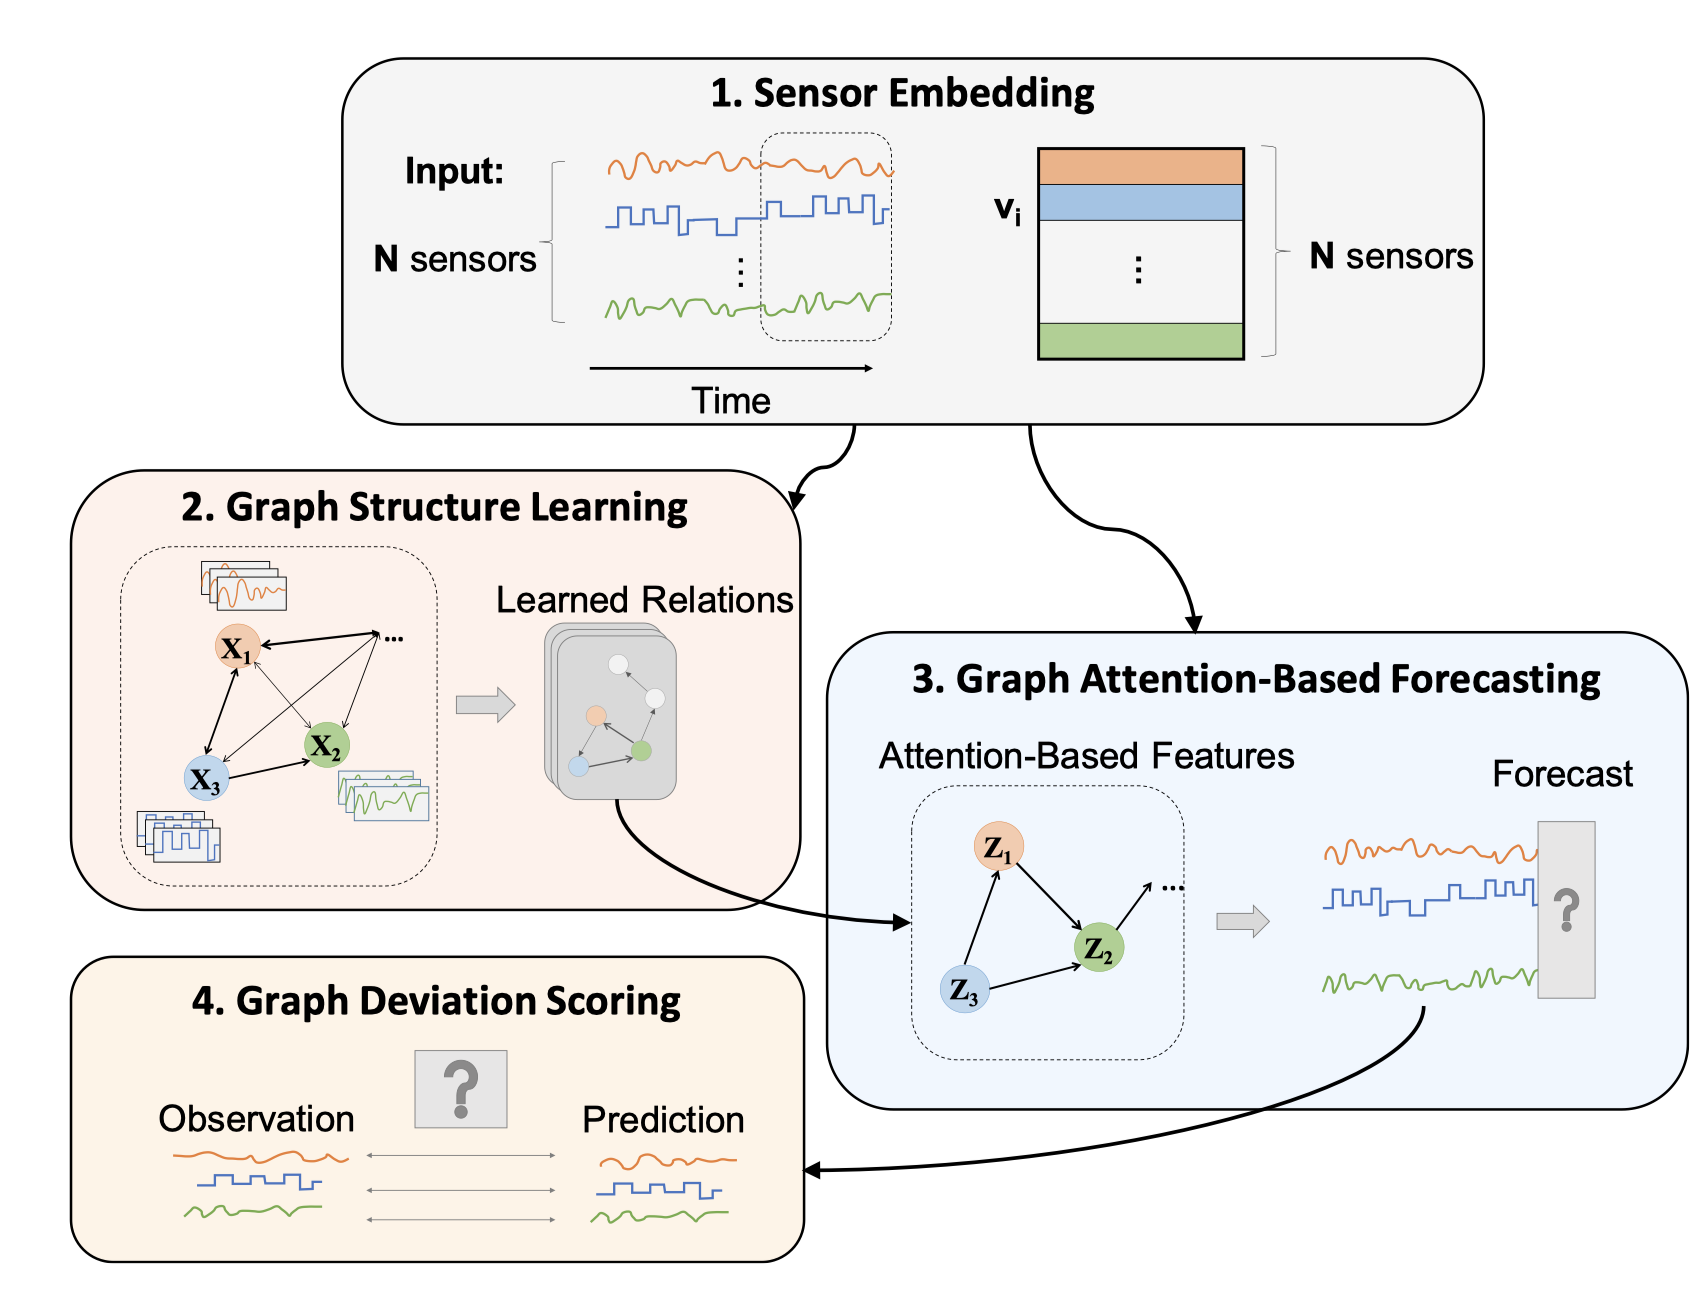
\includegraphics[width = 0.9\textwidth]{chapter1/GDN.jpg}
    \caption{GDN 模型整体架构\cite{gdn}}
    \end{figure}

Dai 等人\cite{ganf}与2022年在ICLR会议上发表了GANF模型。GANF采用 RNN 的方法捕捉时间序列沿时间轴变化的趋势,同时引入贝叶斯网络描述不同时间序列之间的关系,最后采用基于标准化流重建的方式进行异常检测,这种方法更侧重于对时间序列沿时间轴方向变化的特征进行建模。如图所示, GANF 使用了一个贝叶斯网络,并通过 RNN 沿着序列维度对$p(\mathcal{X})$ 进行因子分解 然后使用条件规范化流对时间维度进行因子分解。然后,采用一种新的基于图的依赖性编码器来参数化因子分解产生的条件概率。用于因子分解的 DAG 是一个离散的对象,通常很难学习,但是,离散的结构通过一个可微的图形 $\mathbf { a } $反映在依赖编码器中,这个图形的邻接矩阵就是 $\mathbf { a } $。此外,$\mathbf { A } $必须对应于 DAG 的要求可以表示为一个可微方程。因此,可以通过使用基于梯度的优化来联合优化 $\mathbf { A } $和流组件。
\begin{figure}[htb]
    \centering
    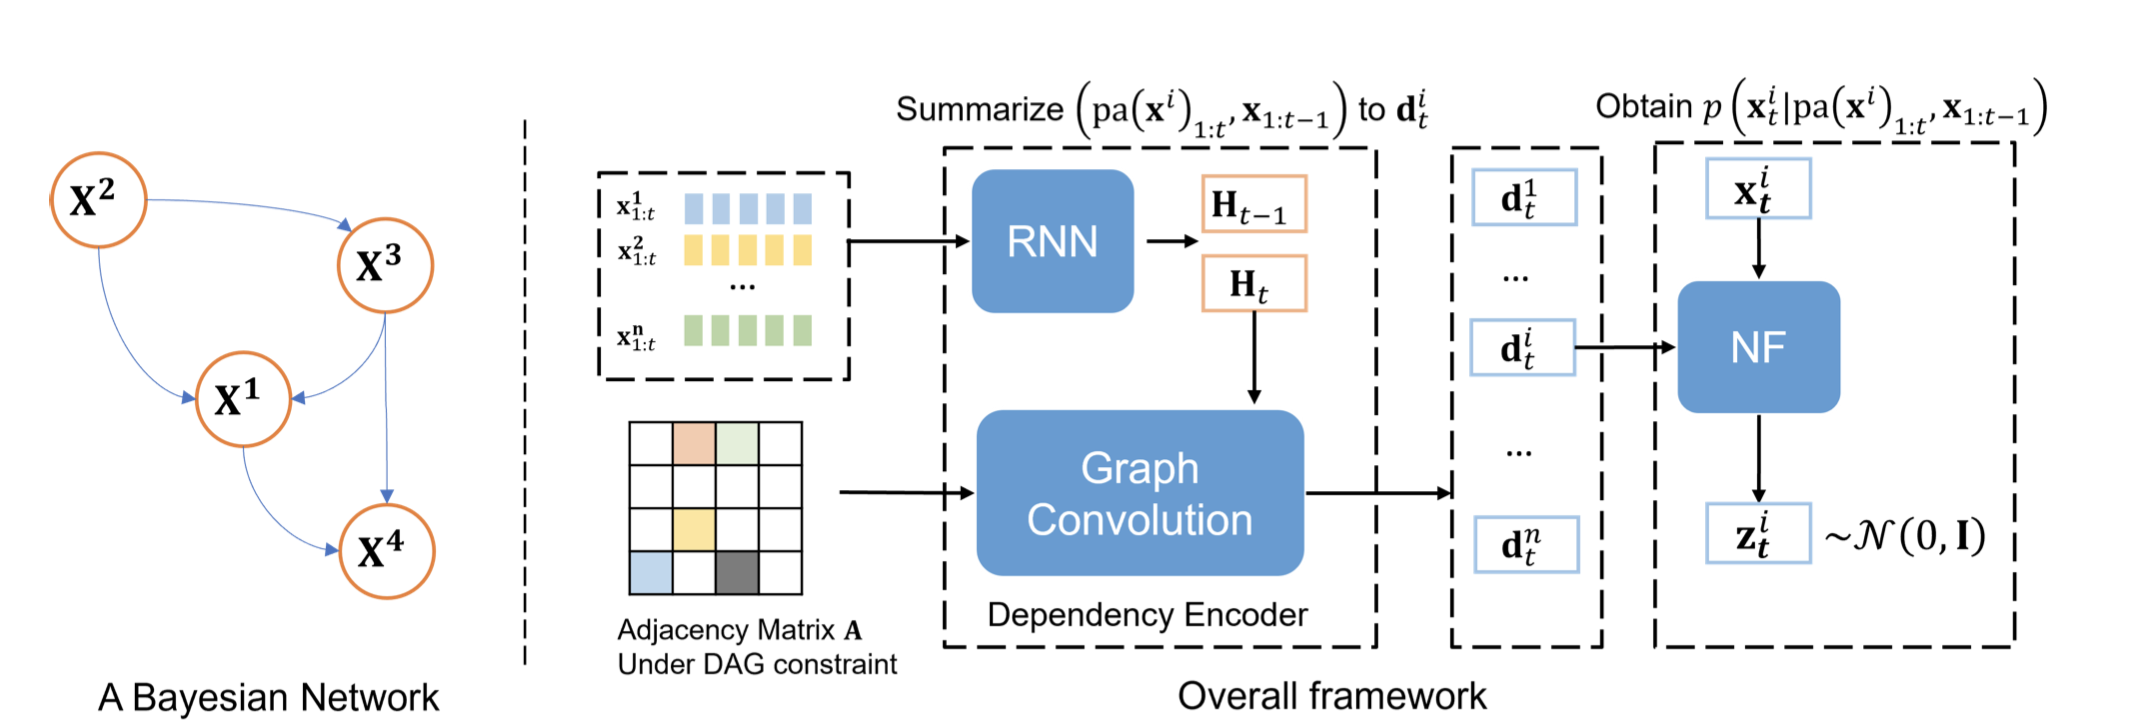
\includegraphics[width = 1\textwidth]{chapter1/GANF.jpg}
    \caption{GANF 模型整体架构\cite{ganf}}
    \end{figure}

\subsection{基于Transformer的时间序列预测异常检测技术}
\begin{figure}[htb]
    \centering
    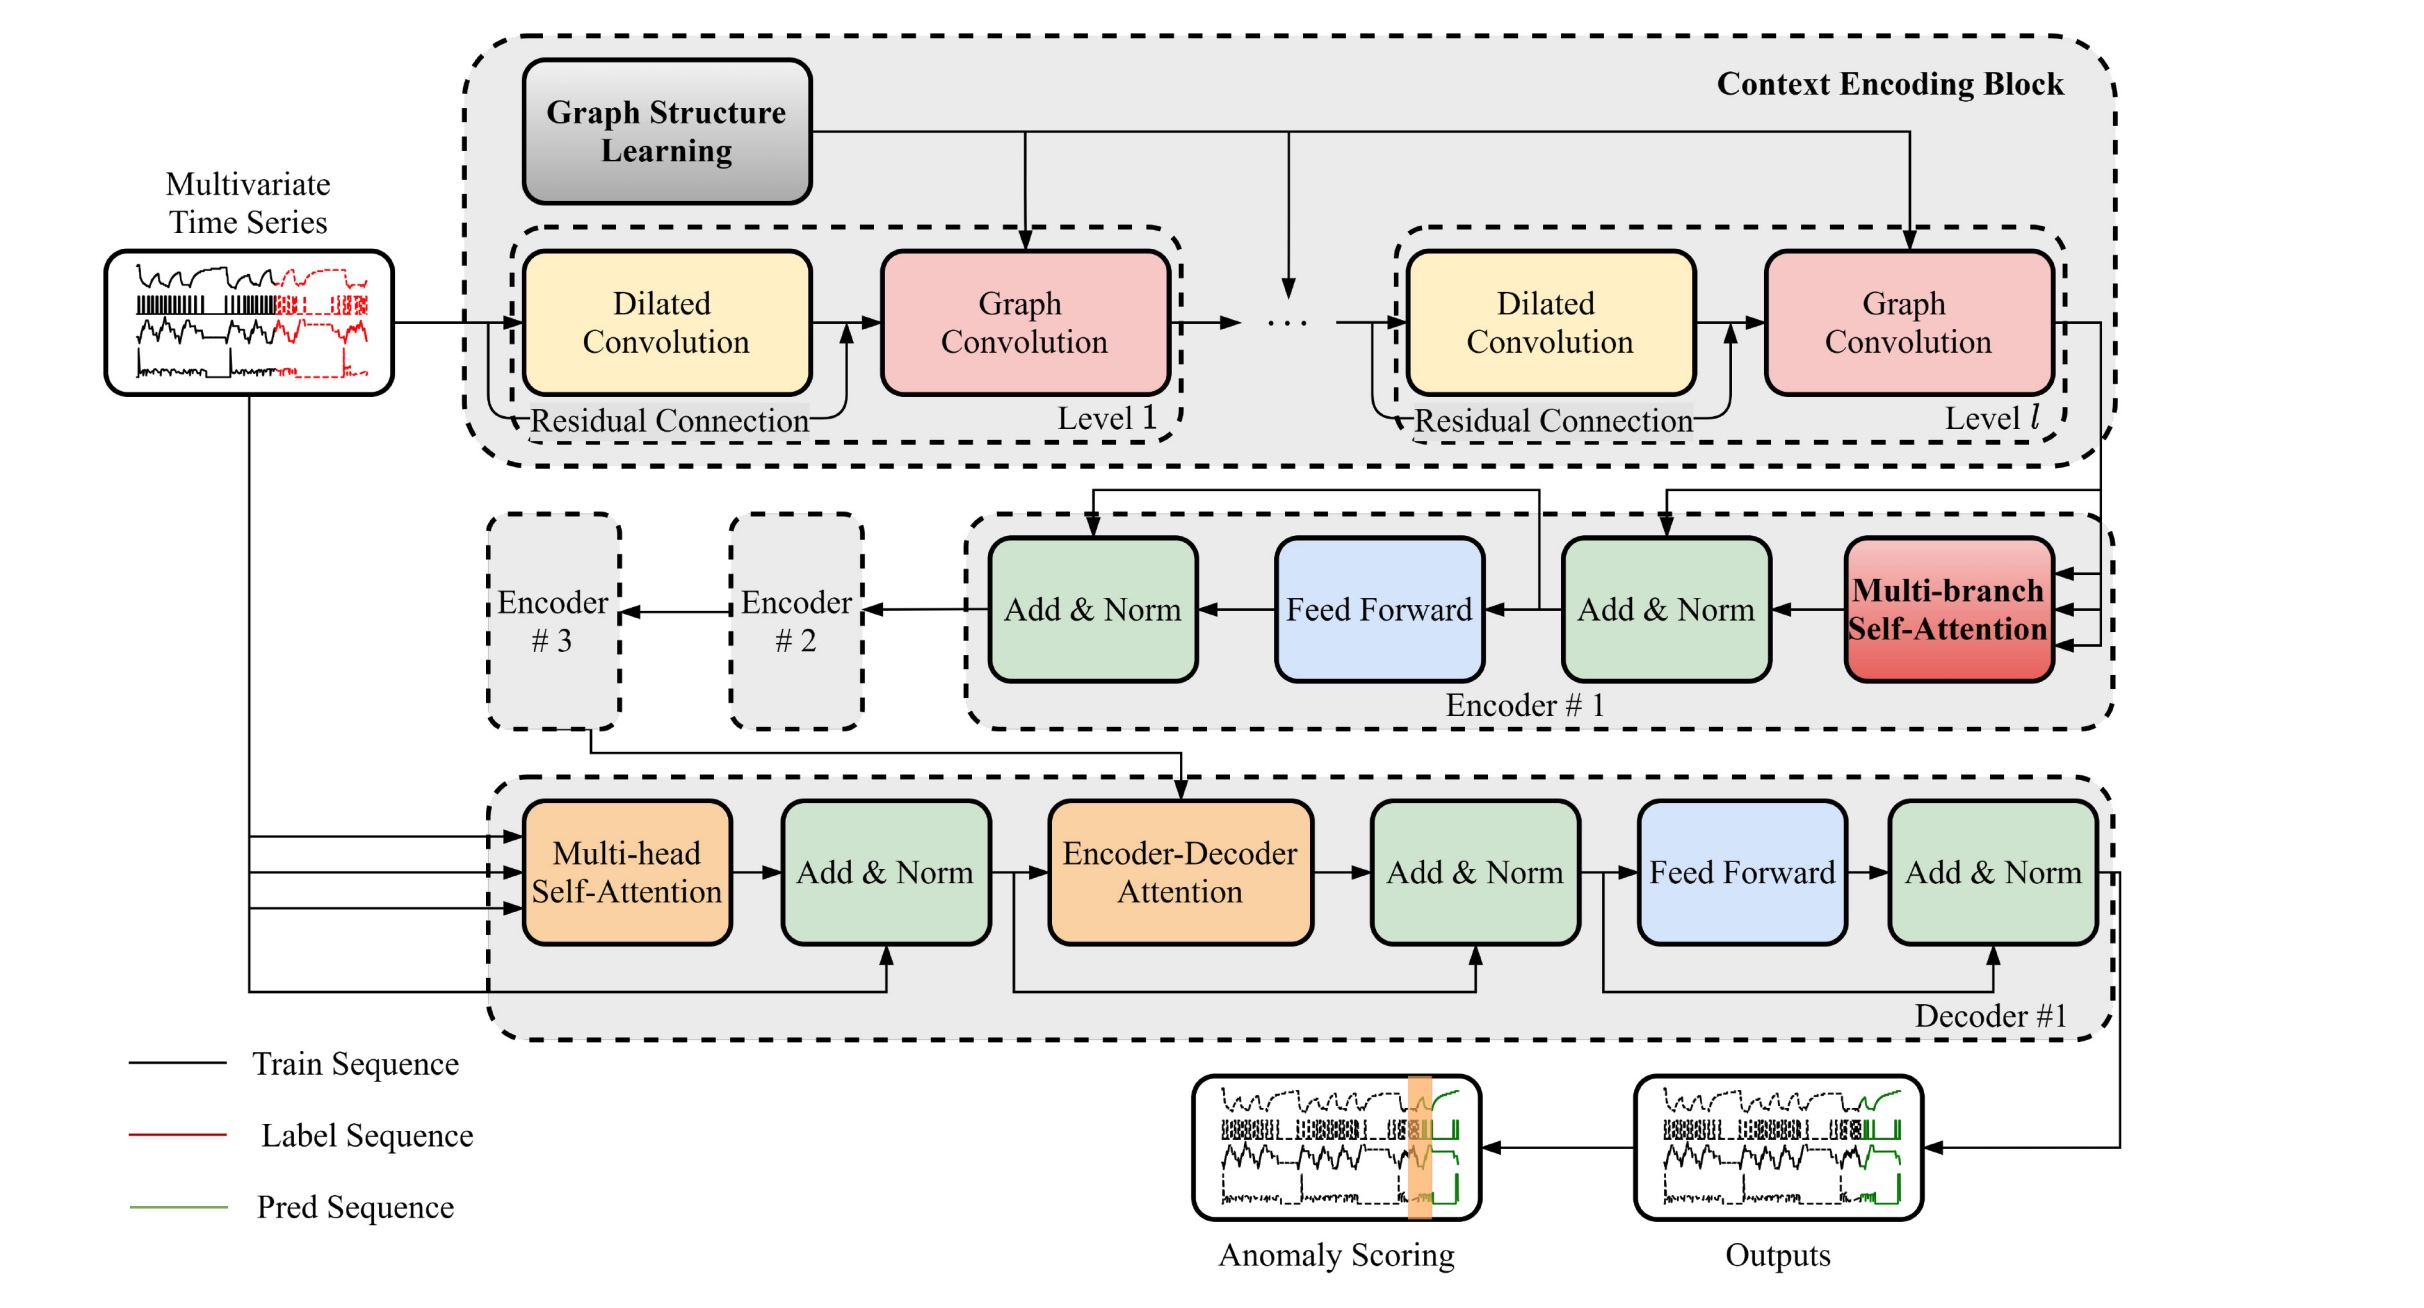
\includegraphics[width = 1\textwidth]{chapter1/gta.jpg}
    \caption{GTA整体架构\cite{gat}}
    \end{figure}
GTA\cite{gat}针对多变量时间序列场景设计Transformer异常检测模型,它们将 Transformer 与基于图形的学习架构相结合。利用了于Transformer的序列建模能力,并采用双向图结构来学习多个物联网传感器之间的关系。提出了一种新的影响传播(IP)图卷积算法,作为传感器之间依赖关系图结构的自动半监督学习策略。作为发现隐藏关系的训练过程的一部分,每个节点的邻域域都受到约束,以进一步提高推理效率。然后,将它们输入到图卷积层中,用于建立信息传播模型。下一步,融合多尺度扩张卷积和图卷积,提供分层的时间上下文编码。它们使用基于转换器的体系结构来建模和预测序列,因为它们具有并行性和捕获上下文信息的能力。作者还提出了一种利用多分支注意降低多头注意二次复杂度的方法。在最近的另一项工作中,他们使用了编码器-解码器叠加结构的变压器,这种结构完全由注意力机制组成。

\section{基于重构的多元时间序列异常检测相关技术}
基于预测的方法在在在某些场景下可能会失效。大多数复杂的时间序列异常检测方法都是建立在对时间序列建模的基础上,以预测未来的数值和预测误差。即便如此,也没有一个稳健的基于预测的模型可以产生一个快速和不断变化的时间序列的精确模型。为了克服基于预测的模型的不足,基于重构的模型可能更有效。基于重构的方法根据其技术又可分为基于AE的方法、基于VAE的方法、基于GAN的方法以及基于Transformer的方法。下文所介绍技术中DAGMM、USAD、APAE属于基于AE的方法;MAD-GAN属于基于GAN的方法;TranAD属于基于Transformer的方法。

\subsection{基于AE的时间序列重构异常检测技术}
DAGMM (深度自动编码高斯混合模型)\cite{dagmm}使用潜在空间中的高斯混合在一个端到端的框架中估计多元时间序列的输入样本概率。该模型由两个主要部分组成: 压缩网络和估计网络。该压缩网络利用随机深度自动编码器对输入样本进行降维处理,根据缩减的空间和重构误差特征产生低维表示。估计网络通过高斯混合模型在低维表示中计算样本能量(下一个定义)。样本能量是用来确定重建误差,高样本能量意味着高度的异常。尽管如此,只考虑了空间依赖性,没有包括时间信息。通过端到端的训练,估计网络引入了一个正则化项,使压缩网络避免了局部最优,并产生了较低的重构误差。然而,它仍然是缓慢的,无法明确利用模态间的相关性。
% \begin{figure}[htb]
%     \centering
%     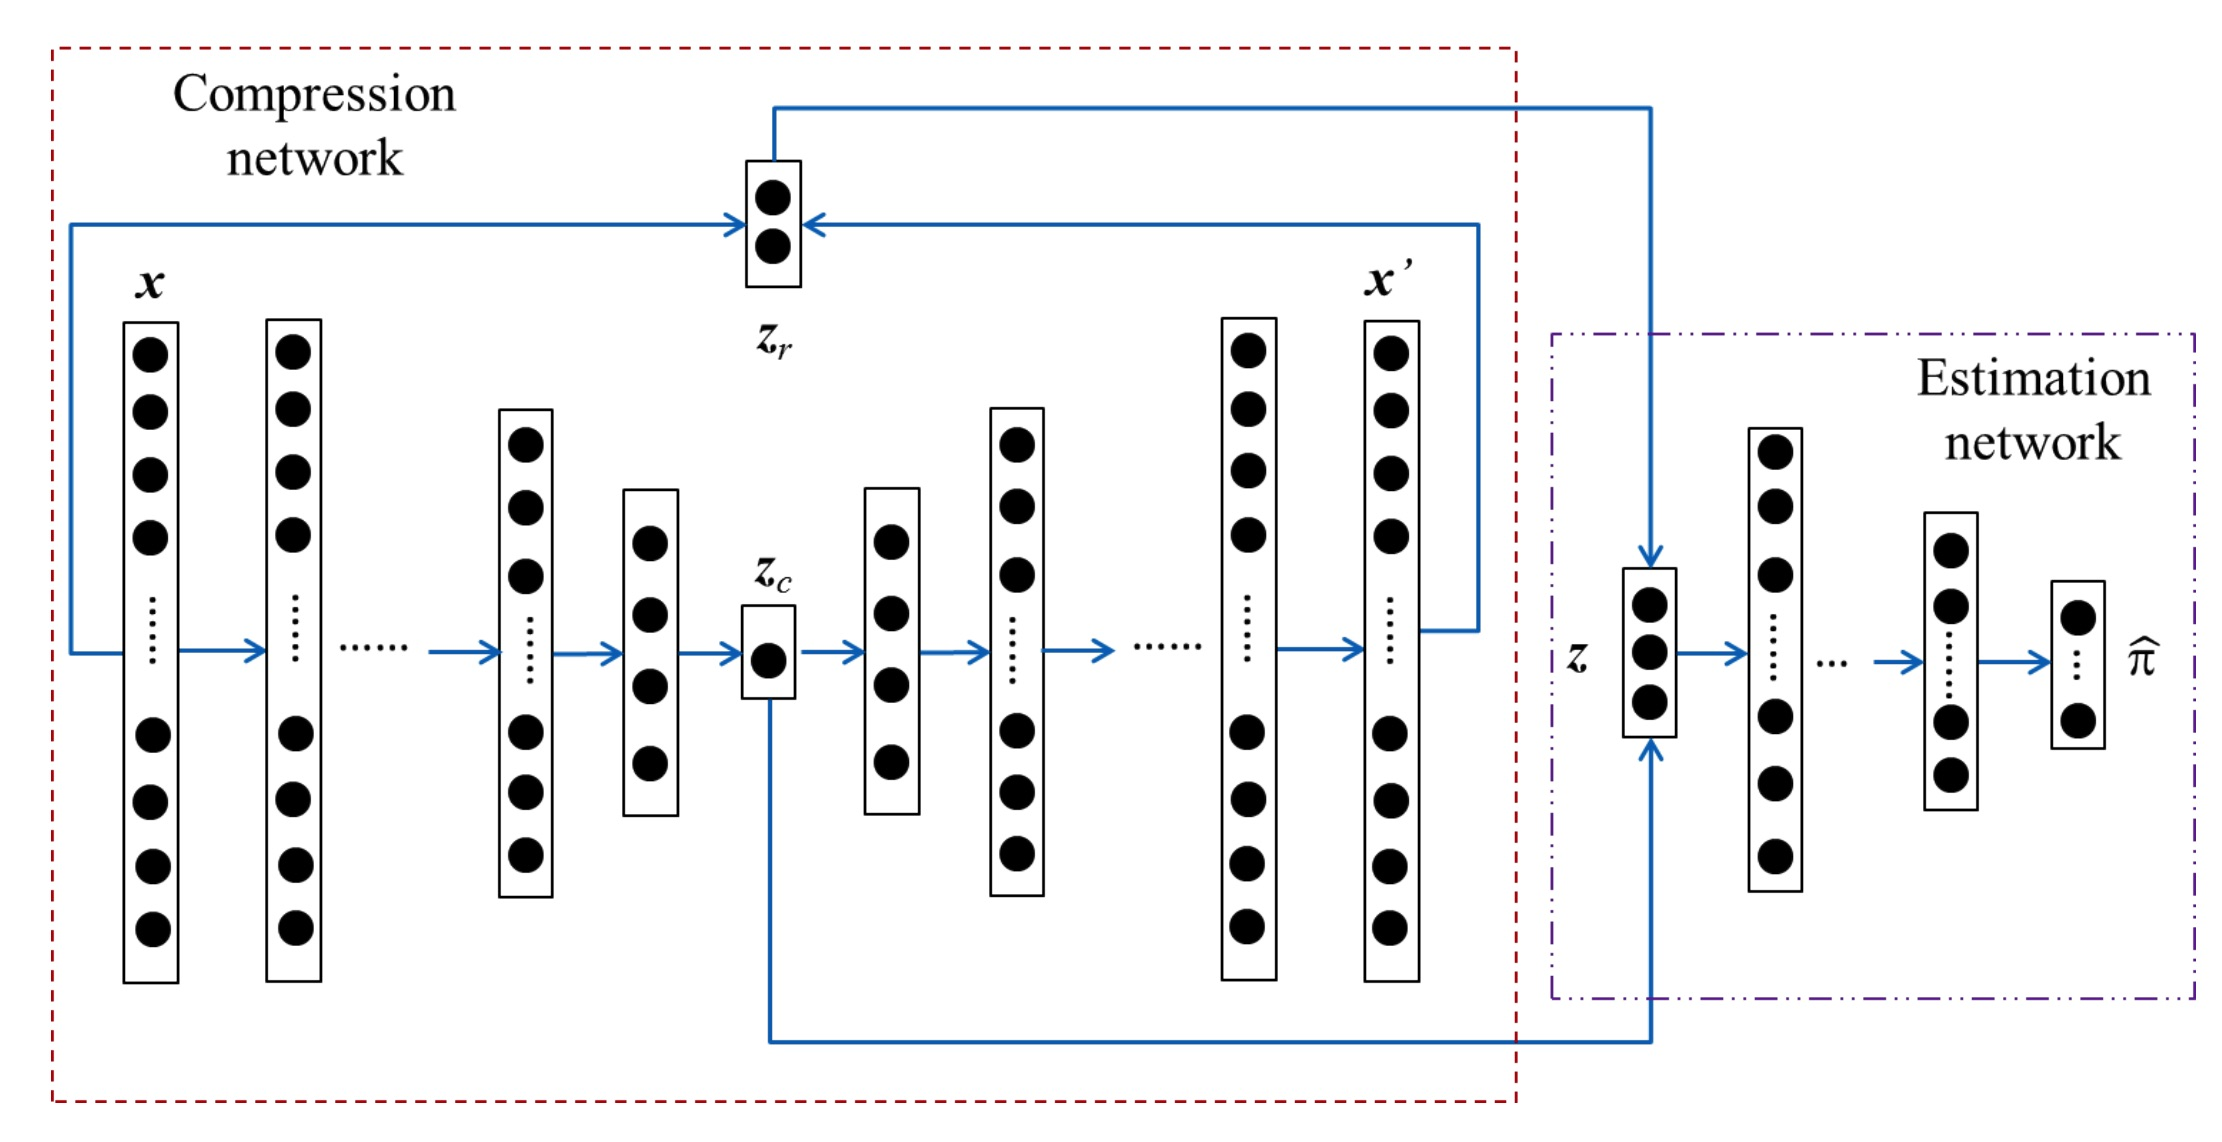
\includegraphics[width = 0.9\textwidth]{chapter1/dagmm.jpeg}
%     \caption{DAGMM模型整体架构\cite{dagmm}}
%     \end{figure}

Audibert等人\cite{usad}在2020年在KDD上发表了USAD模型。USAD基于自动编码器提出了一种基于对抗性学习的重建方法,该方法通过两个自动编码器对抗性学习重建多元时间序列,并以重建值与真实值之间的差异作为异常分数进行异常检测,这种方法更侧重于对数据的整体分布进行建模。同时Audibert等人提出了训练和检测的两种算法。
如图1-3所示,USAD模型具有两个自动编码器 AE1和AE2。 在该模型中自动编码器具有双重目的。其中AE1最小化$W$(阶段1)的重建误差,并最小化AE 2(阶段2)的重构输出之间的差异。随着AE1,AE2 最小化了$W$的重建误差(阶段1),它随后最大化了由AE 1(阶段2)重建的输入数据的重建误差。通过这种对抗性学习的方式,使得USAD模型能够更好的学习到时间序列的分布。在推断阶段, 时间序列的异常分数通过
\begin{equation}
    \mathscr{A}(\widehat{W})=\alpha\left\|\widehat{W}-A E_1(\widehat{W})\right\|_2+\beta\left\|\widehat{W}-A E_2\left(A E_1(\widehat{W})\right)\right\|_2
    \end{equation}
计算得到,其中$\alpha + \beta = 1$并用于参数化误报和真阳性之间的权衡。如果$\alpha$大于$\beta$,则减少真实阳性的数量并减少误报的数量。相反,如果$\alpha$小于$\beta$,以增加假阳性数量的成本增加了真实阳性的数量。则表示α<βA高检测敏感性方案,而$\alpha > \beta$则表示低检测敏感性。这种参数化方案允许使用单个训练的模型在推断中获得一组不同灵敏度异常得分。
\begin{figure}[htb]
    \centering
    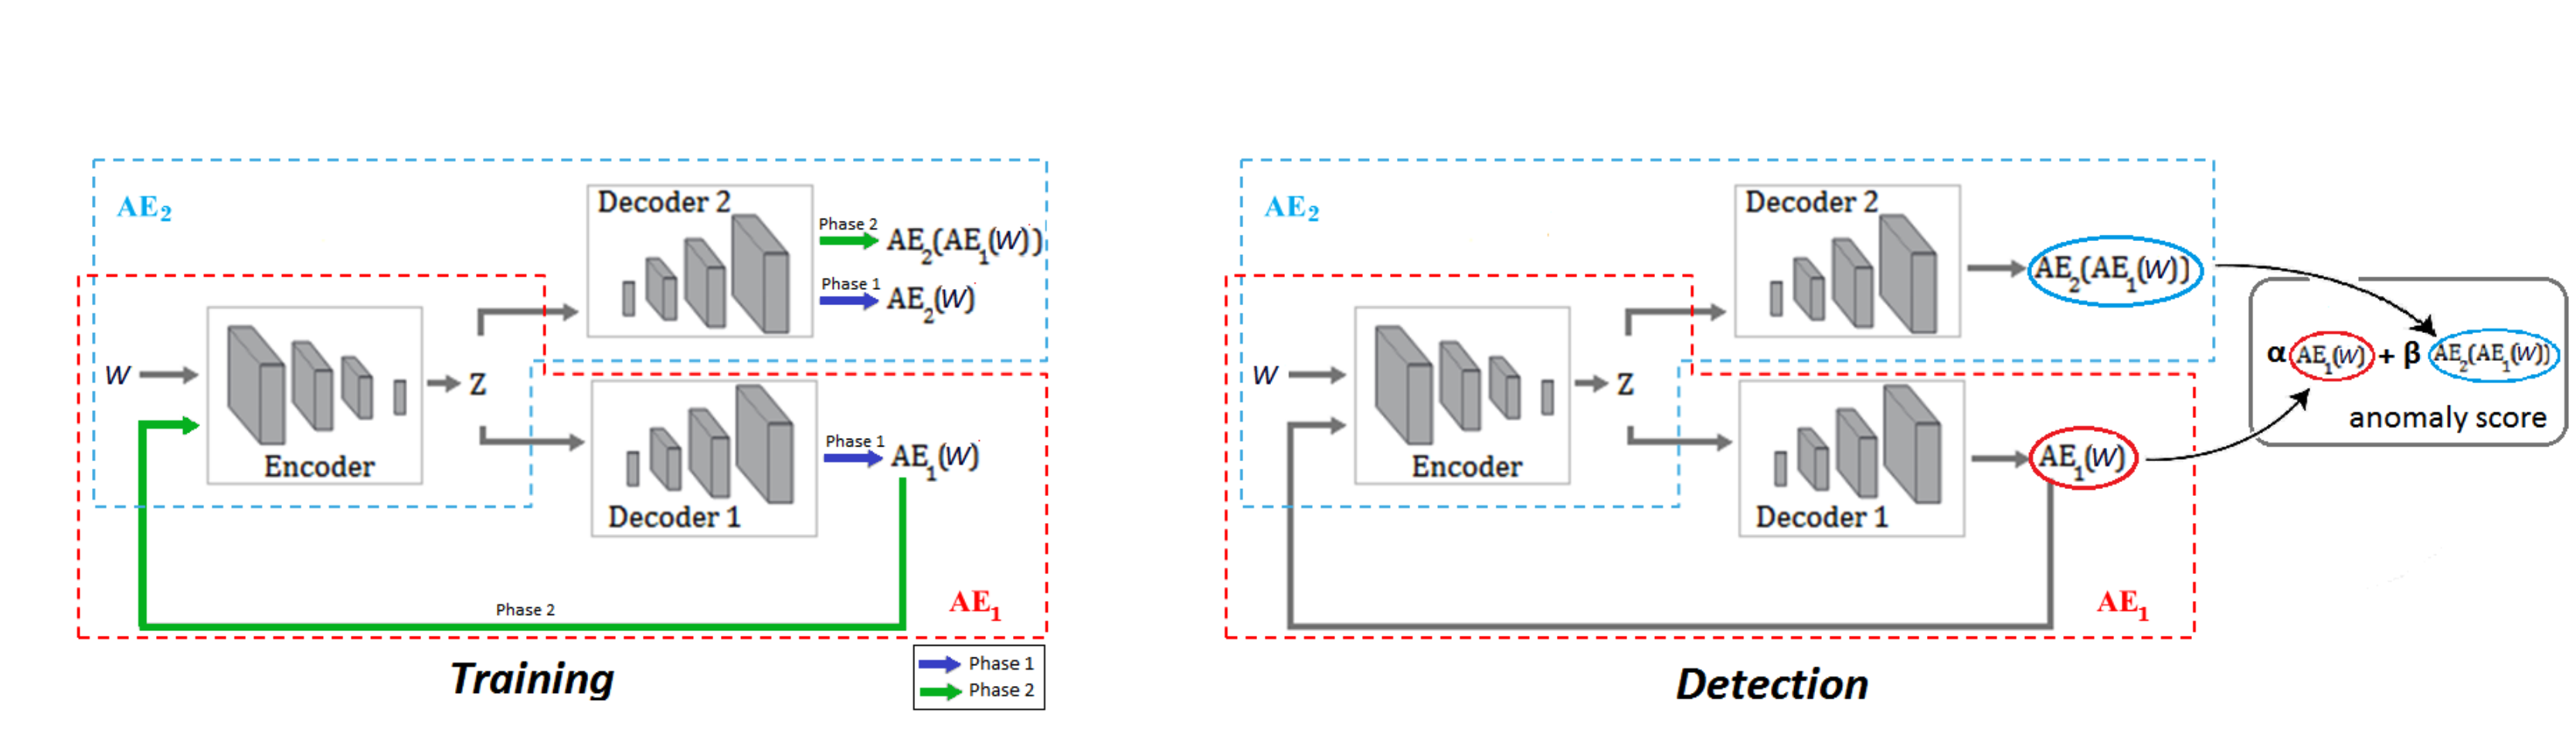
\includegraphics[width = 1\textwidth]{chapter2/usad-overview.jpg}
    \caption{USAD模型整体架构(训练阶段左, 检测阶段右)\cite{usad}}
    \end{figure}

Goodge 等人\cite{apae}通过检查各种对抗性攻击的结果来确定自动编码器是否容易受到异常检测的对抗性攻击。为了提高模型在对手攻击下的性能和鲁棒性,提出了近似投影自动编码器(APAE)。通过对潜在表征使用梯度下降法,这种方法产生了更精确的重建,并增强了对反例威胁的鲁棒性。作为这个过程的一部分,特征加权标准化步骤考虑了不同特征之间重建误差的自然变异性。

% LSTM-VAE\cite{lstm-vae}是一种基于LSTM的变分自动编码器,其采用变分推理进行重建。在原始VAE中,FFN被LSTM代替,LSTM通过去噪自动编码方法训练,以提高表示能力。当给定数据点的对数似然性低于阈值时,该模型检测异常。阈值是动态的和基于状态的,它表示在任务的估计状态上变化的变化阈值,从而可以减少错误警报。
% \begin{figure}[htb]
%     \centering
%     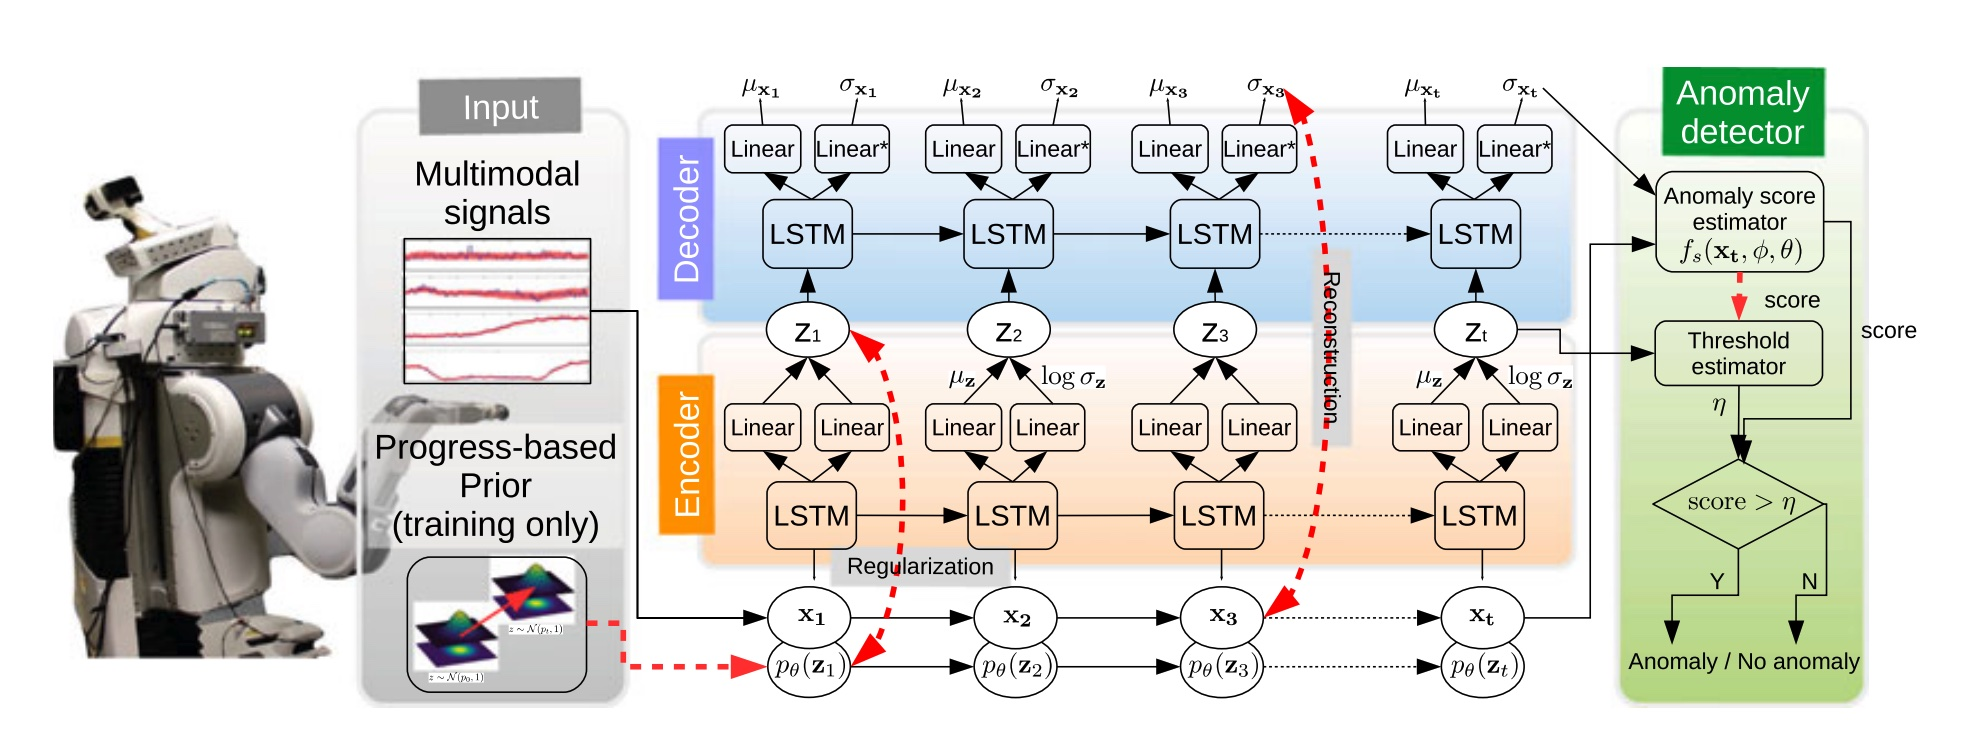
\includegraphics[width = 1\textwidth]{chapter1/lstm-vae.jpg}
%     \caption{LSTM-VAE 总体架构\cite{lstm-vae}}
%     \end{figure}
\subsection{基于GAN的时间序列重构异常检测技术}
多变量异常检测网络(MAD-GAN)\cite{gan}是一个基于通用对抗网络(GAN)的模型。该方法利用 LSTM 作为 GAN 的生成器和鉴别器,同时考虑整个数据,捕捉时间序列分布之间的时间关系。对于异常检测,采用了重构误差和判别损失两种方法。过滤器 GAN 通过在使用伪标签进行训练之前筛选可能的异常样本,减少了传统基于 AE 和基于 GAN 的异常检测模型中过度拟合的问题,从而更准确地捕获正态分布。该生成器还有一个称为自适应权重损失的目标,该目标根据训练过程中不同点的重建误差,动态地为不同点分配权重。通过使用这个训练目标,该模型可以更多地关注合理的正态数据,从而减轻过拟合。
\begin{figure}[htbp]
    \centering
    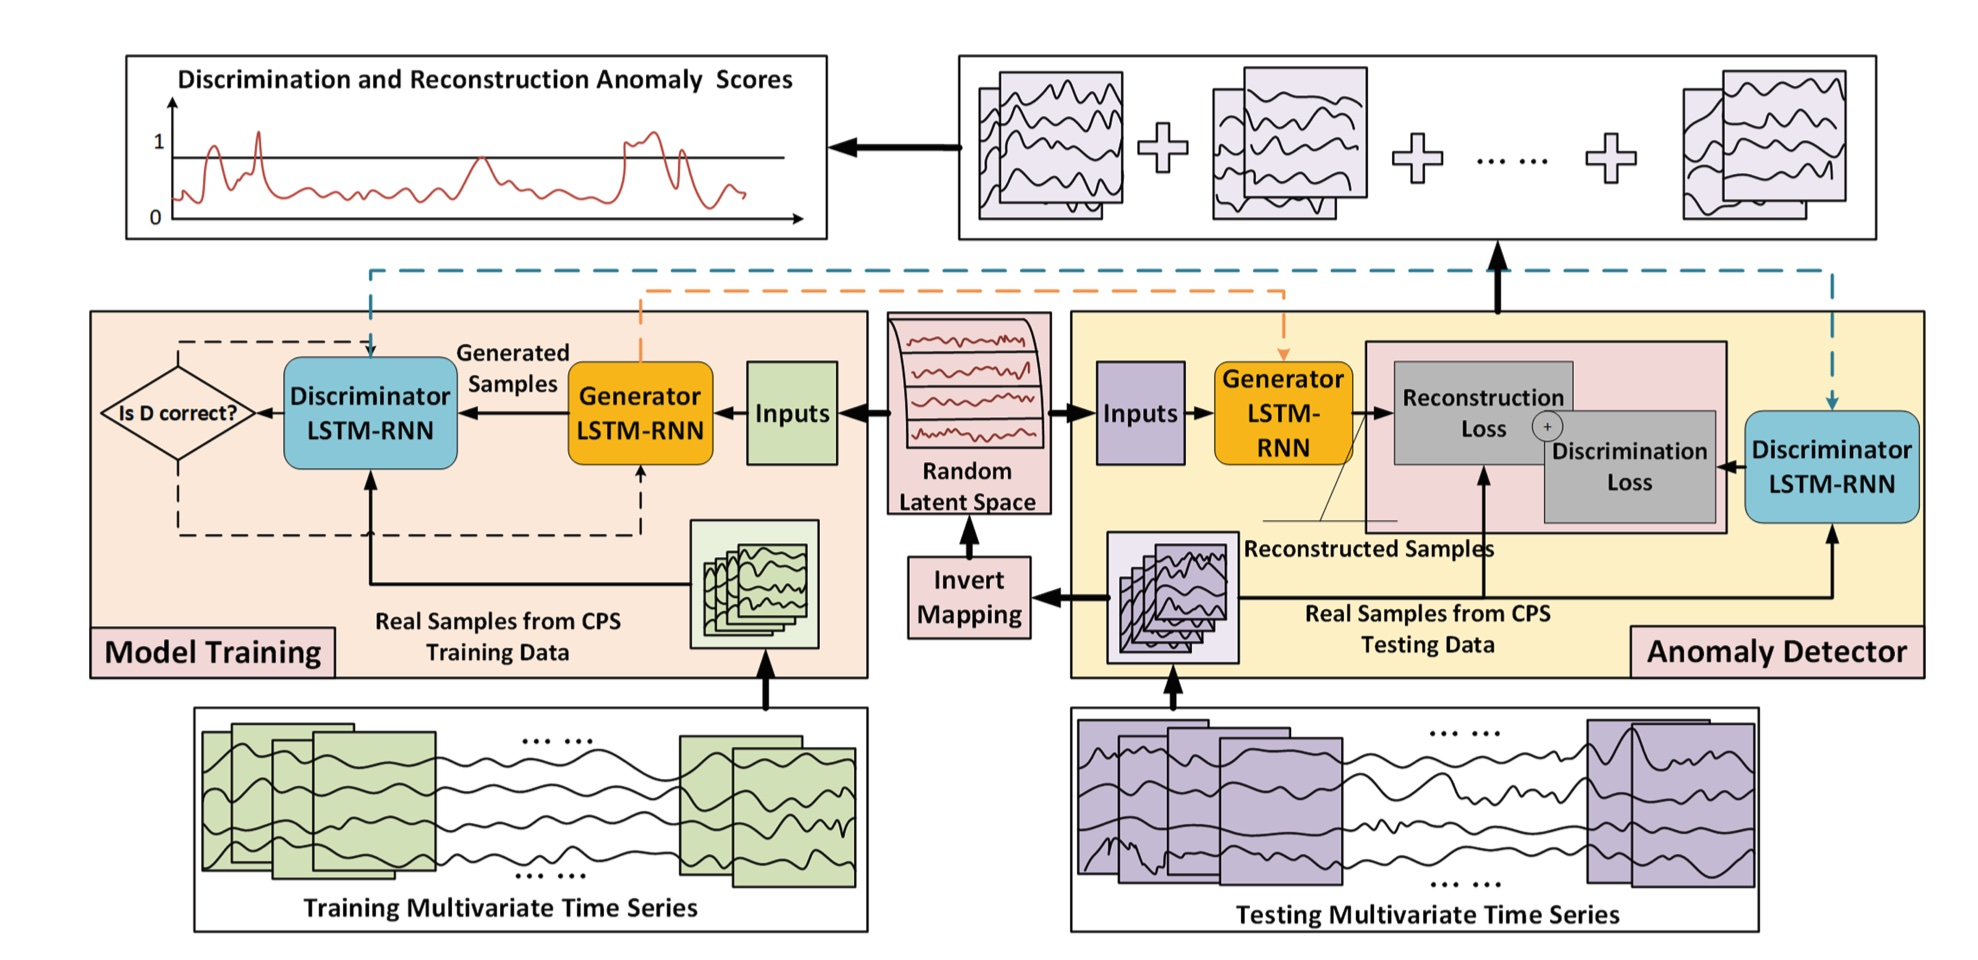
\includegraphics[width = 1\textwidth]{chapter1/mad-gan.jpg}
    \caption{MAD-GAN模型整体架构\cite{mad-gan}}
    \end{figure}

\subsection{基于Transformer的时间序列重构异常检测技术}
TranAD\cite{tranad}是一种基于Transformer的异常检测模型,能够进行自我调节和对抗性训练。由于它的体系结构,在处理大输入时能够有效地进行训练和测试,同时保持稳定性。当偏差太小时,也就是说,如果数据接近正常,基于变压器的编码器-解码器网络可能无法检测异常。该问题可以通过对抗性训练策略来克服,该策略可以放大 TranAD 中的重构误差。
% \begin{figure}[htb]
%     \centering
%     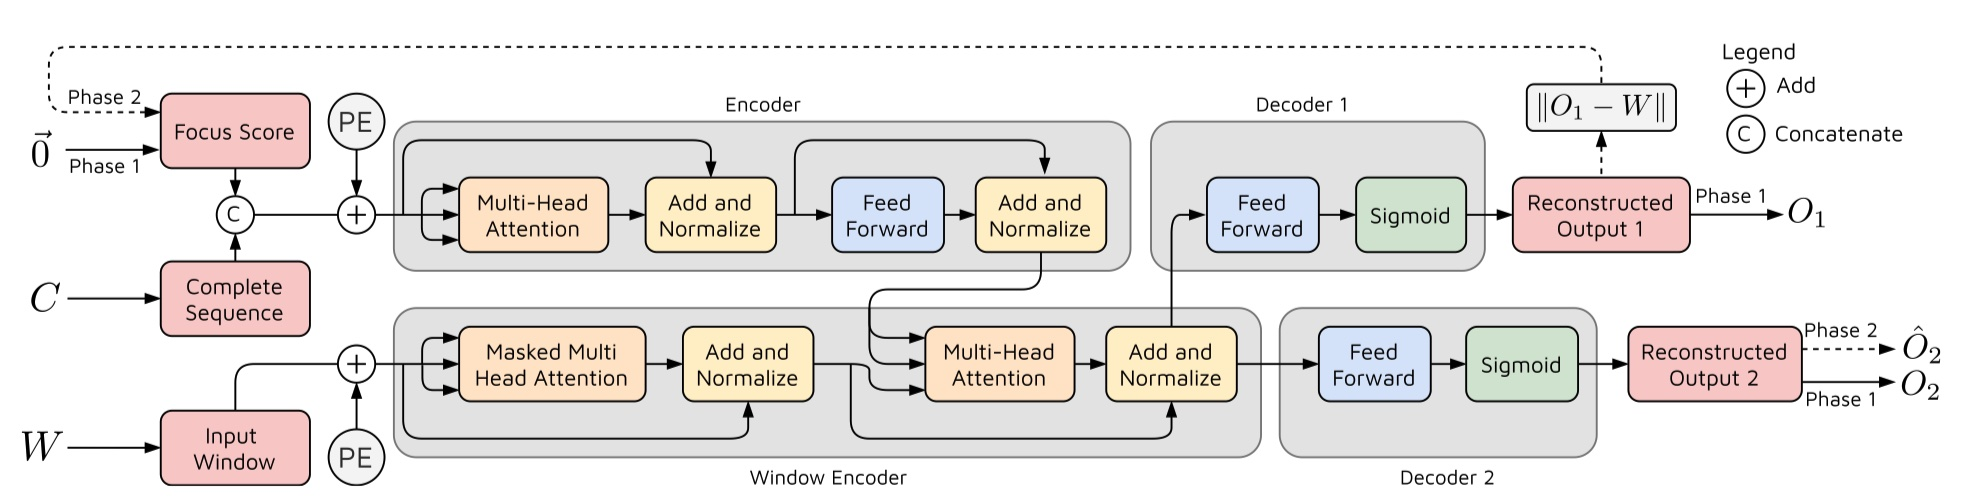
\includegraphics[width = 1\textwidth]{chapter1/tranad.jpg}
%     \caption{TranAD 模型整体架构\cite{tranad}}
%     \end{figure}

\section{本章小节}
本章是多元时间序列异常检测相关背景技术介绍。首先在第一节介绍了什么是时间序列中的异常,即时间序列异常的相关类型,包括全局异常、上下文异常、季节性异常、趋势异常、Shapelet异常等,并通过具体的例子与公式对其进行了详细的解释。然后在第二节和第三节介绍了多元时间序列异常检测的相关技术。在第二节主要介绍了基于预测的多元时间序列异常检测技术及应用,分别介绍了基于RNN的方法、基于CNN的方法、基于GNN的方法以及基于Transformer的方法。在第三节主要介绍了基于重构的多元时间序列异常检测技术,分别介绍了基于AE的方法、基于VAE的方法、基于GAN的方法以及基于Transformer的方法。